\section{Microkernel Architecture}

\begin{frame}{Microkernel Architecture}
    \begin{itemize}
        \item Aufteilung der Anwendung in zwei Arten von Komponenten~\cite{architecturePatterns}
        \item Kern:
        \begin{itemize}
            \item Minimale Funktionalität
            \item Bietet Schnittstelle für Erweiterungen/Plugins
            \item Enthält Plugin-Registry
        \end{itemize}
        \item Module:
        \begin{itemize}
            \item Erweitern Kern um Funktionalitäten
            \item Kommunikation über definierte Schnittstellen
            \item Lose gekoppelt, unabhängig und isoliert voneinander
            \item Verbindung über verschiedene Wege möglich (REST, Messaging, Objekt Instanziierung, \ldots)
        \end{itemize}
    \end{itemize}
\end{frame}

\begin{frame}{Microkernel Architecture: Struktur}
    \begin{figure}[!h]
        \centering
        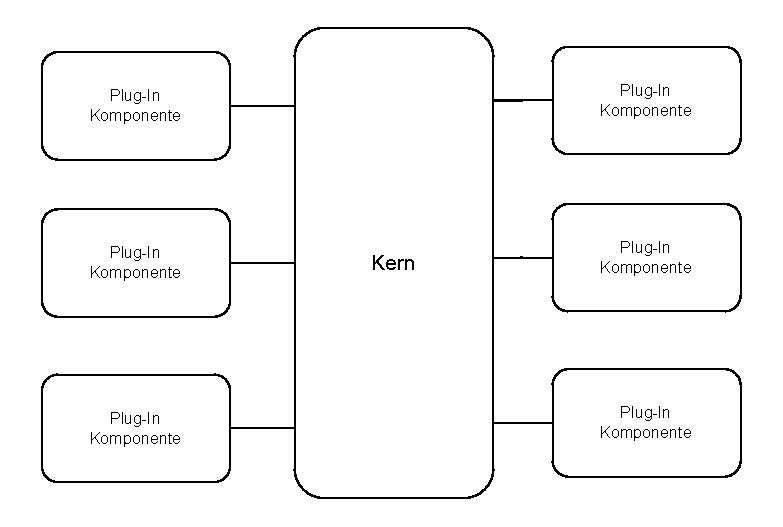
\includegraphics[scale=0.55]{imglib/microkernel/microkernel}
        \caption{Aufbau einer Microkernel Architecture}
        \label{fig:microkernel}
    \end{figure}
\end{frame}

\begin{frame}{Microkernel Architecture: Beispiel E-Commerce I}
    \begin{itemize}
        \item Kern: Großteil der Funktionalität
        \item Module: Auslagerung von Business-Logik zum Bezahlen und Versenden
        \item Einfache Erweiterbarkeit durch neue Dienstleister
        \item Komplexer Kern, hohe Kopplung der übrigen Funktionalitäten
        \item Als einziges Architekturmuster eher nicht geeignet, jedoch in Kombination mit anderen sinnvoll
    \end{itemize}
\end{frame}

\begin{frame}{Microkernel Architecture: Beispiel E-Commerce II}
    \begin{figure}[!h]
        \centering
        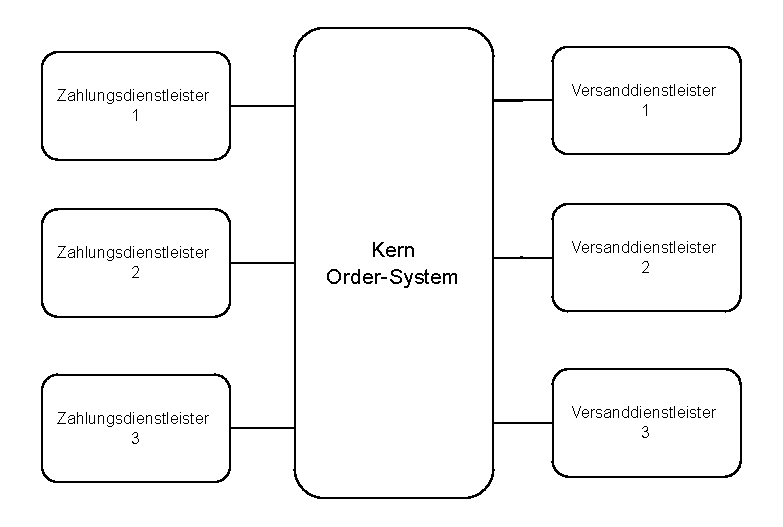
\includegraphics[scale=0.55]{imglib/microkernel/ecommerce-microkernel}
        \caption{E-Commerce-Beispiel mit Microkernel Architecture}
        \label{fig:microkernel-ecommerce}
    \end{figure}
\end{frame}

\begin{frame}{Microkernel Architecture: Agilität}
    \begin{itemize}
        \item Lose Kopplung der Module $\Rightarrow$ schnelle Reaktionsfähigkeit auf Änderungen
        \item Module können einfach ausgetauscht werden $\Rightarrow$ geringe Downtime
        \item Einfach testbar, da Module unabhängig und isoliert voneinander
        \item Kurze Iterationen und Auslieferungszeiten bei Erweiterung der Anwendung
        \item Aber: Hoher initialer Aufwand durch teuren Kern, eher hohe Time-to-Market
        \item Aber: Hoher Aufwand, wenn Kern später Anpassungen benötigt
        \item Fazit: In ausgewählten Anwendungsfällen sinnvoll, aber nicht universell in agilen Umgebungen einsetzbar
    \end{itemize}
\end{frame}
